%%==================================================
%% chapter04.tex for BIT Master Thesis
%% modified by 朱杰
%%==================================================
\chapter{基于稳定标签传播的重叠社区发现算法}

上一章中针对LPA算法的缺陷分析,本文提出了一种基于节点影响力模型的稳定的标签传播算法CDABSLP,然而该算法发现的是非重叠社区,本章将其核心思想引入基于LPA算法改进的重叠社区发现算法--COPRA算法\cite{Gregory2009Finding}之中,试图将其扩展至重叠社区发现领域。多标签传播算法(COPRA)在原始LPA算法的基础上,使得节点可以拥有不止一个标签,这样存在多个标签的节点即代表着隶属于多个社区。但是在保留了LPA算法执行速度快的优点同时,也继承了它不稳定的问题。
% 在验证了上一章所提稳定策略在 LPA 算法上的有效性的基础上,将此稳定策略运用到 COPRA 算法中,以验证其在重叠社区发现算法中的有效性。COPRA 算法\cite{Gregory2009Finding}和 SLPA 算法\cite{Xie2012SLPA}通过允许每个节点拥有多个标签的方法,将 LPA 算法扩展应用于重叠社区的发现,它们既继承了 LPA 算法的优点,也保留了 LPA 算法不稳定和鲁棒性差等缺点。COPRA 算法是最早的基于标签传播的重叠社区发现算法。

多标签传播算法是最早的基于标签传播思想的重叠社区发现算法,本章基于该算法以及上一章提出的CDABSLP算法在稳定性上的设计理念,将提出一种稳定的基于标签传播的重叠社区发现算法(Overlapping Community Detection Algorithm Based on Stable Label Propagation),下文简称OCDABSLP算法。

OCDABSLP算法采用了同步更新标签的策略,这点与CDABSLP算法不同;在标签选择方式上,对于邻居节点标签隶属度均小于既定阈值,且含有多个不同的最大隶属度标签的时候,选择最大隶属度标签中标签影响力模型计算值最大的那一个进行更新。在算法最终收敛之后,根据每个节点含有的标签将其划分到相应的社区,含有多个标签的节点即对应着存在于多个社区的重叠节点。
% 本章将会提出一种基于稳定标签传播的重叠社区发现算法(Overlapping Community Detection Algorithm Based on Stable Label Propagation),下文简称 OCDABSLP。OCDABSLP 算法在迭代执行标签更新过程中,当节点属于所有社区的隶属度都小于阈值且最大值有多个时,选择隶属度最大的多个标签中标签影响强度最大的标签。满足终止条件后,算法根据节点的标签将其划分到相应社区中,拥有多个标签的节点被划分到相应的多个社区中,成为重叠节点,得到最终的重叠社区划分结果。在不同复杂网络数据集上的大量实验表明本章算法能够得到比现有的大部分算法更好的社区划分结果。

%下面这段修改过了
本章接下来的内容组织结构上将先介绍一下多标签传播算法的情况,详细分析COPRA算法目前存在的缺陷;然后详细的阐述OCDABSLP算法在使得多标签传播更加稳定性上的设计;接着是对算法整体执行步骤进行全面的说明,并对算法时间复杂度进行分析; 最后在验证实验部分中,介绍了包括实验环境、实验数据集以及评价指标后,将会详细的分析在人工基准网络上的实验结果,通过与其他基准算法进行对比实验,以此来证明算法的效果。

\section{多标签传播算法的缺陷分析}

多标签传播算法(COPRA)\cite{Gregory2009Finding}最早是由Gregory 等人提出的第一个基于标签传播思想的重叠社区发现算法。COPRA算法是一种模糊性重叠社区发现算,它允许节点拥有不止一个标签,但是每个标签同时还需对应着一个隶属度,即代表着该节点隶属于该标签的模糊比例。
% Gregory 等人\cite{Gregory2009Finding}提出的 COPRA 算法是第一个利用标签传播思想进行重叠社区发现的算法。算法中每个节点可以以不同隶属度拥有多个标签,每个节点包含一组标签-隶属度对$(l, b)$,$l $表示节点所属社区的编号,$b $表示节点属于该社区的隶属程度,$b_t(l, i)$表示在第$ t $次标签传播结束时节点$ i $属于社区$ l $的隶属程度。COPRA 通过迭代地更新各个节点的标签及隶属度来获取社区结构。

与 LPA 算法相同,初始时,COPAR 算法为每个节点分配一个各不相同的标
签,并将其隶属度设置为 1,即 $b_0(i, i) = 1$。然后采用同步更新策略进行标签更新
迭代,在每次更新过程中,用邻接点中出现的所有相同标签的平均隶属度更新该
节点的标签-隶属度对列表。每一轮更新后,删除隶属度小于 $\frac{1}{v}$ 的标签($v$ 是算法的参数),当一个节点的所有标签对应的隶属度都小于 $\frac{1}{v}$ 时,就只保留一个
隶属度最大的标签,若此时有多个标签的隶属度同时取最大值,就随机保留隶属
度最大的标签中的一个,然后对所有剩余标签的隶属度进行归一化。更新结束后,
算法根据节点的标签将其划分到相应的社区中。一个节点最后拥有的标签数即为
它被划分到的社区的个数。 

函数 $b_t(l, i)$用于计算在第 $t $次迭代中,节点$ i $属于社区$ l $的隶属程度,计算如
公式\ref{eqn:lishudu}所示。

\begin{equation}
  \label{eqn:lishudu}
  b_t(l,i)=\frac{\sum_{j\in \Gamma_i }b_{t-1}(l,j)}{d_i}
\end{equation}

COPRA 算法的执行过程如算法\ref{alg:COPRA}所示。

\begin{algorithm}[htb]  
  \caption{多标签传播算法(COPRA)}  
  \label{alg:COPRA}  
  \begin{algorithmic}[1]  
    \Require  
    复杂网络 $G = (V, E)$,最大迭代次数 $maxIter$   
    \Ensure  
      社区划分结果;  
    \State 初始化,为网络中的每个节点分配一个各不相同的标签,标签-隶属度对集合为${(i,l)}$;
    
          令迭代次数$t=0$;  

    \State 标签传播迭代过程:

    (a)如果迭代次数 $t > maxIter$,标签传播迭代过程结束,转 Step3;
    
    否则继续算法。 

    (b)对于每个节点$v_i\in V$,根据公式\ref{eqn:lishudu}计算该节点属于其邻接点集合中出现的所有标签的隶属度,更新标签-隶属度对列表。
    
    根据参数$v$删除不满足条件的标签,并对剩余标签进行归一化。 
     
    (c)如果连续两次迭代结束后,标签集合的大小不变,那么标签传播迭代过程停止,
    转Step3;
    
    否则,令$t = t+1$转到步骤(a)继续执行。

    \State 社区划分,将拥有相同标签的节点划分到同一个社区中,不同标签的种类就表示网络中社区的个数。
  \end{algorithmic}  
\end{algorithm} 

COPRA 算法继承了 LPA 算法的优点,也保留了 LPA 算法稳定性和鲁棒性差等缺点,且容易把所有项点分配给一个社区,有些时候还可能会划分出一些无意义的社区。

\section{算法核心思想}

\subsection{同步更新标签}

在CDABSLP算法中使用的是异步更新标签,为的是防止标签传播过程中产生震荡,且加快收敛速度,但是那是在非重叠社区发现中的有效手段,而在重叠社区发现算法中,由于节点本身就具有多标签,因此不会出现LPA算法中才会遇到的标签震荡问题。如若使用异步更新标签,在多标签传播过程中,甚至反而会导致标签混乱,致使最终结果出现失真现象,不具有复现性。

综上所述,在本章提出的OCDABSLP算法中,将会延续使用同步更新标签的策略。

\subsection{标签选择阶段的改进}

原始COPRA算法中的唯一一个不稳定因素是当节点属于所有社区的隶属度
都小于阈值且最大值有多个时,会随机选择一个标签。因此,在此处对 COPRA
算法进行改进。当出现上述情形时,选择隶属度最大的多个标签中标签影响力
最大的标签。当标签影响力最大的标签仍有多个时,保留所有标签影响强度最
大的标签。标签影响强度的计算如公式\ref{eqn:LI2}所示。

\begin{equation}
  \label{eqn:LI2}
  NI(i,l)=\sum_{j \in \Gamma _i} b_{t-1}(l,j) \frac{NI(j)}{d_j}
\end{equation}

\section{算法整体流程}

基于以上两项稳定性设计原则,本章提出的OCDABSLP算法的在整体上主要可以分为初始化阶段、标签传播阶段两大部分。在标签传播阶段之后实际上还应有一个社区划分阶段,但是标签传播迭代完毕,网络中存在的每个标签即对应着一个社区,相应标签的节点即为属于该社区的节点,因此实质上,在标签传播结束就已经得到了相应的社区划分,后续唯一需要做的就是统计一下节点标签,将所有节点归类至相应社区,故本小节未将社区划分单独列为主要内容进行说明。图\ref{fig:ocdabslp}为 OCDABSLP 的算法流程图。

\begin{figure}
  \centering
  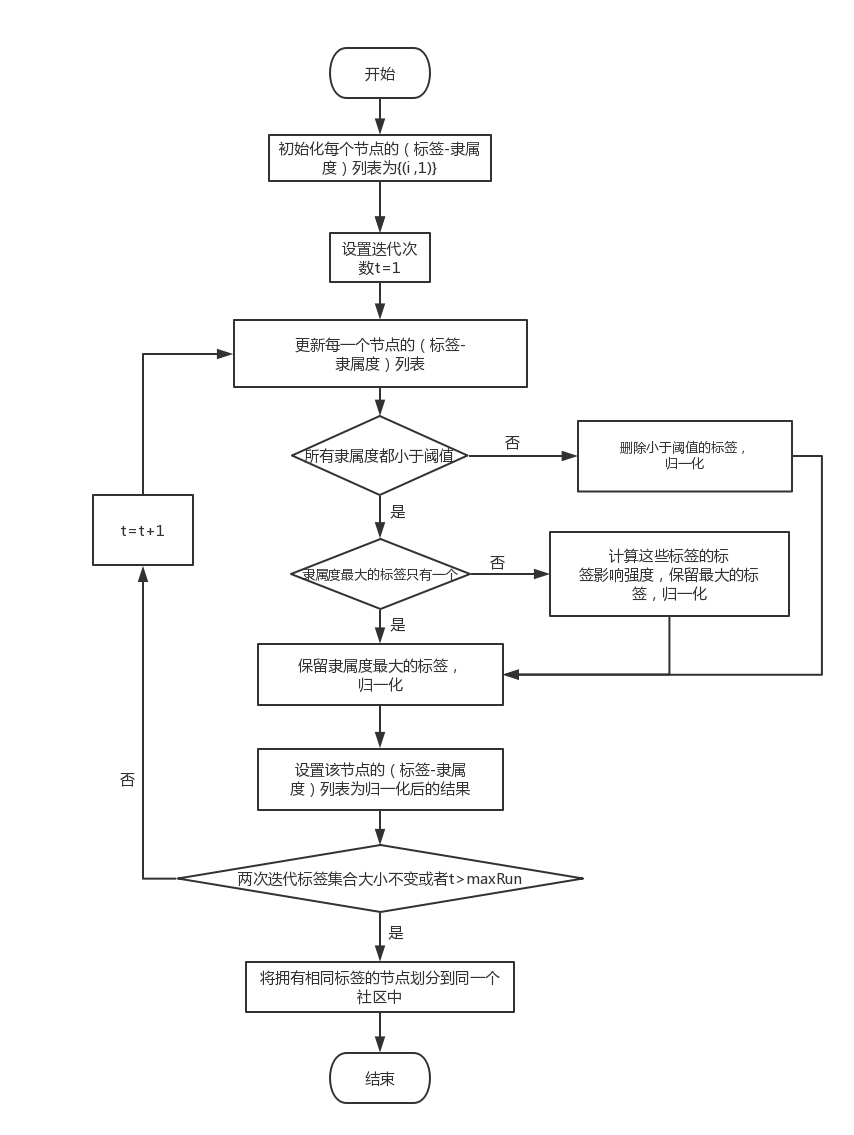
\includegraphics[width=1\textwidth]{figures/ocdabslp}
  \caption{OCDABSLP算法流程图}\label{fig:ocdabslp}
\end{figure}

\subsection{初始化阶段}

在算法的初始化阶段中:
\begin{enumerate}
  \item 初始化每个节点的(标签-隶属度)列表为$ \{ (i,1) \} $;
  \item 对网络进行k-核分解,获取所有节点的k-核值$Ks(i)$,并在计算时,将中间过程中统计得出的每个节点的度保留下来以备下一步使用;
  \item 通过节点影响力公式\ref{eqn:NI}在初始化阶段计算每个节点的节点影响力,以备后续计算标签影响力大小使用;
  \item 将所有节点以节点影响力大小的降序进行排列后加入标签更新队列,节点影响力相同的节点,按照节点ID号升序排列。
\end{enumerate}
CDABSLP算法初始化阶段具体可参考算法\ref{alg:OCDABSLPchushihua}。

\begin{algorithm}[h]  
  \caption{OCDABSLP算法初始化阶段}  
  \label{alg:OCDABSLPchushihua} 
  \begin{algorithmic}[1]  
    \Require  
      社交网络$G=(V,E)$,节点影响力可调参数$\alpha$,标签隶属度阈值参数$v$;  
    \Ensure  
      所有节点的影响力,标签更新队列;  
    \State 初始化每个节点的(标签-隶属度)列表为$ \{ (i,1) \} $;  
    \State 对网络G进行k-核分解,获取所有节点的k-核值$Ks(i)$; 
    \State 通过节点影响力公式计算每个节点的节点影响力; 
    \State 将所有节点以节点影响力大小的降序进行排列后加入标签更新队列,节点影响力相同的节点,按照节点ID号升序排列; 
  \end{algorithmic}  
\end{algorithm}  

\subsection{标签传播阶段}

在算法的标签传播阶段中:
\begin{enumerate}
  \item 更新每一个节点的(标签-隶属度)列表;
  \item 若隶属度不都小于阈值,删除小于阈值的标签,并进行归一化;
  \item 若隶属度都小于阈值且隶属度最大的标签唯一,是则保留隶属度最大的标签,并进行归一化;
  \item 若隶属度都小于阈值且隶属度最大的标签不唯一,计算这些标签的标签影响强度,保留最大的标签,并进行归一化;
  \item 设置该节点的(标签-隶属度)列表为归一化后的结果;
  \item 不断迭代直至标签不再更改或者已经达到最多迭代次数。
\end{enumerate}
CDABSLP算法标签传播阶段具体可参考算法\ref{alg:OCDABSLPlpa}。

\begin{algorithm}[h]  
  \caption{OCDABSLP算法标签传播阶段}  
  \label{alg:OCDABSLPlpa} 
  \begin{algorithmic}[1]  
    \Require  
      所有节点的影响力,标签更新队列,最大允许迭代轮数$maxIter$;  
    \Ensure  
      多标签传播结果;  
    \State 迭代次数$iter=1$;  
    \Repeat  
      \State 更新每一个节点的(标签-隶属度)列表;
      \If{所有隶属度都小于阈值}  
        \If{隶属度最大的标签唯一}  
          \State 保留隶属度最大的标签;  
        \Else  
          \State 计算这些标签的标签影响强度,保留最大的标签;
        \EndIf
      \Else  
        \State 删除小于阈值的标签
      \EndIf
      \State 归一化;
      \State 设置该节点的(标签-隶属度)列表为归一化后的结果;  
    \Until{$iter > maxIter$ \textbf{or} 标签不再改变}
  \end{algorithmic}  
\end{algorithm}

\section{算法时间复杂度分析}

OCDABSLP算法的时间复杂度情况如下:

\begin{itemize}
  \item 所有节点初始化标签所花费的时间为$O(N)$;
  \item 标签迭代中的普通标签传播所花费的时间为$O(v \cdot M \cdot log(v \cdot \frac{M}{N}))$;
  \item 标签迭代中若遇到节点所属社区的隶属度都小于阈值且最大值有多个时,计算标签影响力所花费的时间为$O(v \cdot M \cdot log(v \cdot \frac{M}{N}))$;
  \item 社区划分过程所花费的时间为$O(N)$;
\end{itemize}

综上,OCDABSLP算法的整体时间复杂度为:$2 \cdot O(N)+2t \cdot O(v \cdot M \cdot log(v \cdot \frac{M}{N}))$;其中N,M,t分别表示节点总数、边的总数以及标签传播过程迭代次数,通常迭代次数不会很多,即相对于社交网络中N和M的大小,t一般仅是一个常数。可见OCDABSLP算法依然保持着很高的执行效率。

% \section{算法时间复杂度分析}
% OCDABSLP 算法的时间复杂度分析如下: 

% (1)为每个节点初始化标签所用时间复杂度为$ O(|V|)$; 

% (2)每次标签传播过程分为两部分: 传统的标签传播过程:$O(v|E|log(v|E|/|V|))$;当节点属于所有社区的隶属度都小于阈值且最大值有多个时,利用
% 公式\ref{eqn:LI2}计算标签影响值的过程:$O(v|E|log(v|E|/|V|))$; 

% (3)将相同标签的节点划分到一个社区的时间复杂度为 $O(|V|)$。 

% 标签传播过程是不断迭代执行的,因此整个算法的时间复杂度为
% $2O(|V|)+2tO(v|E|log(v|E|/|V|))$。

\section{验证实验}
本节为本章提出的基于稳定标签传播的重叠社区发现算法OCDABSLP算法进行实验验证。首先介绍实验的软硬件环境和采用的数据集,然后对算法的评价指标进行简单阐述,最后是相关对比实验的结果展示与分析。

\subsection{实验环境}
本文实现的OCDABSLP算法所使用的软硬件环境与上一章节的CDABSLP算法一致,机器配置如表\ref{tab:tab3-1}所示。OCDABSLP算法使用Python语言编程实现,均基于Python的复杂网络相关软件包Networkx,使用Anaconda来对软件包进行管理和部署,具体配置如表\ref{tab:tab3-2}所示。

\subsection{数据集}
选用4组不同的LFR基准网络人工生成数据集进行实验验证本章所提算法的有效性。 

LFR基准网络是目前在社区发现领域使用最多的人工数据集之一。通
过调整网络生成参数可以产生用户需要的不同的人工数据集,LFR 基准网络的主
要生成参数及其含义在上一章节中已经提及,如表\ref{tab:tab3-4}所示。

本节实验将生成四组具有重叠社区结构的 LFR 基准网络数据集,详细的生成参数如
表\ref{tab:tab4-1}示。 

\begin{table}
  \centering
  \caption{四组重叠LFR基准网络生成参数} \label{tab:tab4-1}
  \begin{tabular*}{0.9\textwidth}{@{\extracolsep{\fill}}ccccccccc}
  \toprule
    编号		&N  &avgk &maxk &minc &maxc &mu &on &om\\
  \midrule
    S7	&10000  &15 &500 &10 &500 &0.1 &100 &$2\sim 8$\\
    S8 &10000  &15 &500 &10 &500 &0.3 &100 &$2\sim 8$\\
    S9 &50000  &15 &500 &20 &1000 &0.1 &100 &$2\sim 8$\\
    S10 &50000  &15 &500 &20 &1000 &0.3 &100 &$2\sim 8$\\
  \bottomrule
  \end{tabular*}
\end{table}

\subsection{评价指标}
本章采用重叠 NMI(ENMI)\cite{Lancichinetti2009Detecting}和重叠模块度 EQ
\cite{Lancichinetti2010Finding}作为重叠社区发现结果的评价指标。下面介绍这些指标。

(1)EQ

在上一章节已经提到了模块度的概念,而重叠社区模块度(EQ)\cite{Lancichinetti2010Finding}可以在其公式\ref{eqn:modular}的基础上修改为公式\ref{eqn:modular2}。

\begin{equation}
  \label{eqn:modular2}
  Q=\frac{1}{2m} \sum_{k=1}^c \sum_{i,j \in C_k} \frac{1}{O_iO_j} \left [ A_{ij}-\frac{k_ik_j}{2m} \right ]  
\end{equation}

在公式\ref{eqn:modular2}中,i和j表示网络中的两个节点,m表示网络中边的数量,$k_i$和$k_j$表示节点i和j的度数,$O_i$和$O_j$表示节点i和j所属的社区的个数,A表示网络的邻居矩阵,$C_k$表示网络的第k个社区。该公式的数学意义为:网络中同一社区内部的边的比例与在同样社区结构下的基准网络内部边的比例的期望值之差。模块度越高,则网络中社区划分结果越好。


(2)ENMI

在上一章节已经提到了NMI的概念,而ENMI\cite{Lancichinetti2009Detecting}是在其重叠社区上的扩展,具体计算方式详见公式\ref{eqn:enmi}。

\begin{equation}
  \label{eqn:enmi}
  NMI(X,Y) = 1 – \frac{1}{2} [H(X|Y)_{norm} + H(Y|X)_{norm}]
\end{equation}

其中$H(X,Y)$函数表示联合熵,X和Y分别是一个社区,$H(X \mid Y)$函数表示条件熵。

\subsection{实验结果及分析}

(1)人工基准网络上的实验

为了验证本章提出的稳定策略用在 COPRA 算法中的效果,进行本组实验,
将 OCDABSLP 算法与 COPRA 算法进行比较。图\ref{fig:S7ENMI}$\sim$\ref{fig:S10ENMI}中的八幅图分别是
OCDABSLP 算法和 COPRA 算法在四组重叠 LFR 基准网络数据集(S7$\sim$S10)上
实验结果的 ENMI 和 EQ 指标的对比图。实验中,参数 v 设置为 om 的值。由于
COPRA 算法存在随机性,因此取 10 次实验的平均值作为最后的结果。横轴代
表重叠节点所属的社区个数 om,取值从 2 到 8;左侧四幅图的纵轴代表社区划
分结果的 ENMI 值,右侧四幅图的纵轴表示实验结果的 EQ 值。 

\begin{figure}
  \centering
  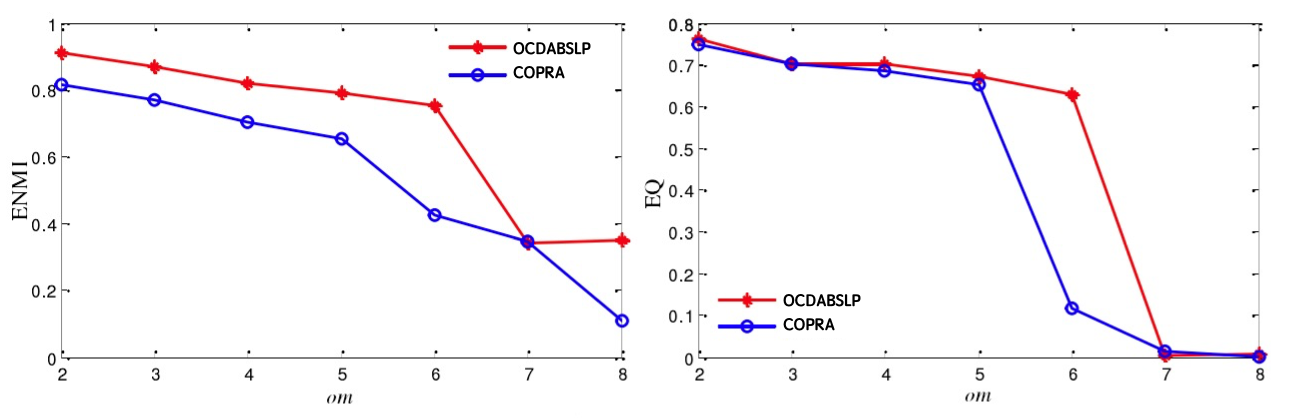
\includegraphics[width=0.75\textwidth]{figures/S7ENMI}
  \caption{在S7网络上的实验结果的ENMI和EQ比较}\label{fig:S7ENMI}

  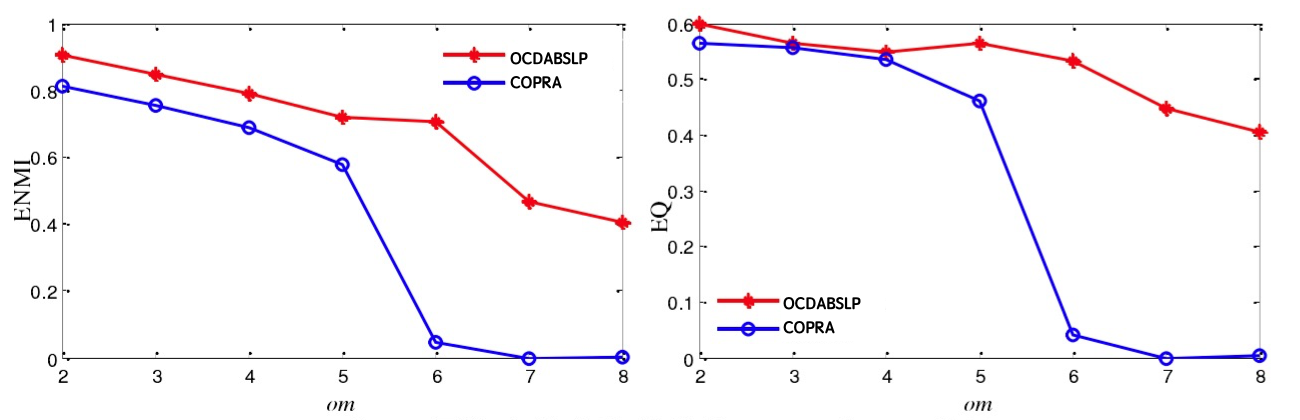
\includegraphics[width=0.75\textwidth]{figures/S8ENMI}
  \caption{在S8网络上的实验结果的ENMI和EQ比较}\label{fig:S8ENMI}

  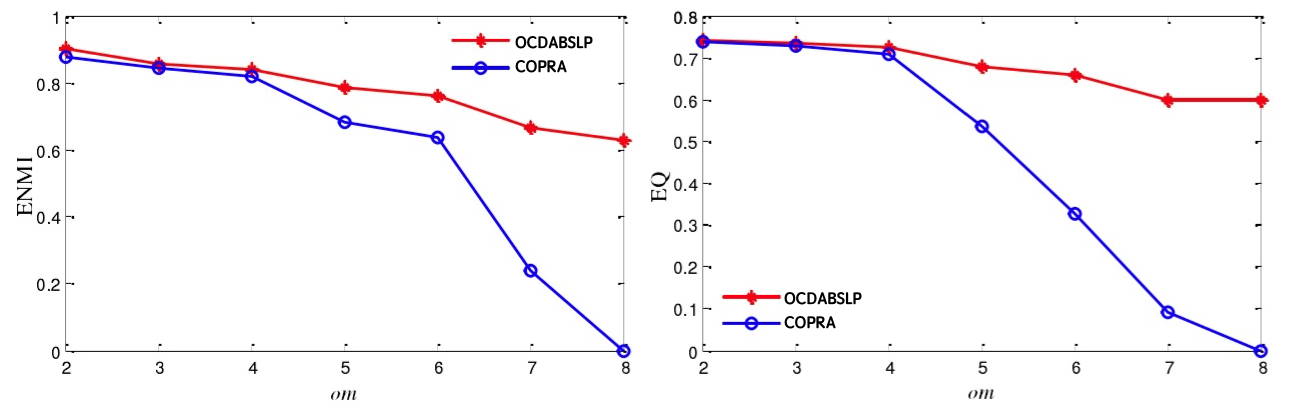
\includegraphics[width=0.75\textwidth]{figures/S9ENMI}
  \caption{在S9网络上的实验结果的ENMI和EQ比较}\label{fig:S9ENMI}

  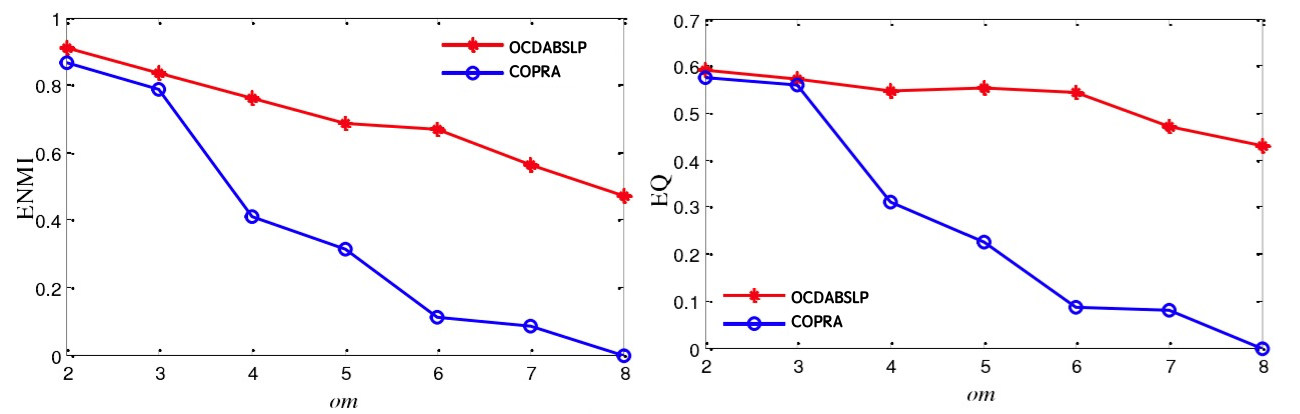
\includegraphics[width=0.75\textwidth]{figures/S10ENMI}
  \caption{在S10网络上的实验结果的ENMI和EQ比较}\label{fig:S10ENMI}

\end{figure}

从图\ref{fig:S7ENMI}$\sim$\ref{fig:S10ENMI}中可以看出,ODABSLP 算法不仅能够得到稳定的社区发现结果,
而且得到的社区结构 ENMI 和 EQ 两个指标都优于 COPRA 算法。验证了本章所
提方法在重叠社区发现方面能得到比较好的结果。

% (2)可视化对比

% 待加入。。。


% \subsection{实验总结}

% OCDABSLP 算法采用同步更新策略,在标签更新过程中,当一个节点拥有
% 的所有标签对应的隶属度都小于 1/v,且此时有多个标签的隶属度同时取最大值
% 时,将节点影响值引入到标签隶属度计算公式中,得到这些标签的影响强度,保
% 留影响强度最大的标签,取代传统 COPRA 算法随机保留其中一个标签的方法,
% 提高算法的稳定性。在重叠 LFR 数据集上的实验结果表明 OCDABSLP 算法解决
% 了 COPRA 算法不稳定的问题,能够检测得到较优的重叠社区结构,验证了本章
% 提出的稳定策略在重叠社区发现算法 COPRA 算法中的适用性。

\section{本章小结}
本章主要介绍了一种基于稳定标签传播的重叠社区发现算法,简称OCDABSLP。OCDABSLP 算法采用同步更新策略,在标签更新过程中,当一个节点拥有
的所有标签对应的隶属度都小于 1/v,且此时有多个标签的隶属度同时取最大值
时,将节点影响值引入到标签隶属度计算公式中,得到这些标签的影响强度,保
留影响强度最大的标签,取代传统 COPRA 算法随机保留其中一个标签的方法,
提高算法的稳定性。在重叠 LFR 数据集上的实验结果表明 OCDABSLP 算法解决
了 COPRA 算法不稳定的问题,能够检测得到较优的重叠社区结构,验证了本章
提出的稳定策略在重叠社区发现算法 COPRA 算法中的适用性。